\documentclass{article}
\usepackage{graphicx}

\title{Comparison between insertionsort, quicksort, radixsort, heapsort and hybridsort.}
\author{Giray Sahin}

\begin{document}
\maketitle
\section{Introduction.}
Our target comparisons sortings on the data requested by the program or the user and see the cases.

We compare 5 comparison-based sorting algorithms: insertionsort, quicksort, radixsort, heapsort and hybrid sort(created by us).

\subsection{Instertion Sort}
Insertion sort is one of the sorting algorithms and is basically used to sort the elements in an array from smallest to largest (or largest to smallest). This algorithm works by going through the elements sequentially and adding each element to its appropriate place.

The first element is considered sequential. In this case, the first element of the array is considered sequential. Other elements are added at the appropriate location within the ordered section. The new element moves from the end of the sequential section to the appropriate position. At each step, the new element is compared with the previous elements and placed in the appropriate position.
This step is repeated until all elements in the array are placed inside the ordered part.

Basic time complexity of the algorithm $O(n^2)$ and n represents the number of elements of the array. However, if the data set is relatively small and a large portion of the list is already sorted, the performance of the algorithm may be better.

\begin{center}
\begin{tabular}{|c|c|c|}
 \hline
Best Case & Avarage Case & Worst Case  \\
\hline
$O(n)$ &$ O(n^2)$ & $O(n^2)$ \\
\hline
\end{tabular}
\end{center}

Especially if the array sorted in an ascending order, we will have the best case. In such a case, the complexity
of insertion sort is $O(n)$.

\subsection{Quick Sort}
Quick sort is one of the sorting algorithms and is known for its fast performance. This algorithm is based on the "divide and conquer" strategy and uses a recursive approach.

Quick sort has 4 steps: 
Pivot Selection: An element in the array is selected and this element is called "pivot". Pivot selection can be done with a variety of strategies, but usually the element in the middle of the array or a random element is selected.

Partition: Other elements in the array are compared with the pivot, and those smaller than the pivot are placed on the left, and those larger than the pivot are placed on the right. As a result of this step, the pivot element finds the correct position of the sequential array.

Recursive Sort: Left and right subarrays (except pivot) are treated the same. That is, both subarrays implement pivot selection, splitting and recursive sorting steps within themselves.

Merging: Once the subarrays are sorted, we get the fully sorted array by merging the sorted subarrays.


\begin{center}
\begin{tabular}{|c|c|c|}
 \hline
Best Case & Avarage Case & Worst Case  \\
\hline
$O(nlog(n))$ &$ O(nlog(n))$ & $O(n^2)$ \\
\hline
\end{tabular}
\end{center}

However, in some cases (e.g. in case of poor pivot choice) the worst case time complexity
It could be $O(n^2)$. Pivot selection strategies can be developed to prevent this situation.

\subsection{Radix Sort}
Radix sort is one of the sorting algorithms and is used to sort numbers. Specifically, it sorts by the digits of each element. It is also known as "radix-based sorting".
It gives us the desired order by checking the numbers from the smallest digit to the largest. After sorting starting from the lowest digit, proceed to the next digit and repeat the process. This step continues until the highest step is reached.\\

The time complexity of this algorithm is usually
It is expressed as $O(nk)$, where
n is the number of elements to be sorted,
k represents the number of digits.

\subsection{Heap Sort}
Heap Sort is one of the sorting algorithms developed to keep data in order in memory. Clipping sort creates a heap tree in the background and sorts by taking the number at the top of this tree. (Please remember that the largest number in the stack tree will always be at the top.)

The Sort transforms the given array into a max heap structure, then extracts the root element from the max heap and adds it to the sorted partition, and rebuilds the max heap structure with the remaining elements; It repeats this process until there are no elements left in the max heap.


Heapsort is one of the "in-place" sorting algorithms, that is, it performs the sorting process without using any additional memory. Also in worst case, average case and best case scenarios

It has $O(nlog(n))$ time complexity. Heapsort is especially useful in situations where there is no need for dynamic sorting where elements are added and removed.

\subsection{Hybrid Sort}

The hybrid sorting algorithm is a sorting algorithm created by us and written based on our tests of the time complexity of the insertionsort, quicksort, radixsort and heapsort sorting algorithms (the fact that it is based on our tests means that a better hybridsort algorithm can be written). Hybrid sorting algorithm dynamically sorts data by input.  As an example: suppose, that radixsort is better than quicksort for some arrays (say, for arrays with > 1000 elements). Then the hybrid sorting algorithm uses radix to sort arrays with larger than 1000 elements, and quicksort for the smaller arrays. 


\maketitle
\section{Methodology}
The algorithms were implemented in C++. We compared insertionsort, quicksort, radixsort and heapsort. Then, based on the comparison, we implemented the best hybrid sorting algorithm(based on our tests).
For all algorithms were given the same input data and tested on arrays of sizes 



\maketitle
\section{Results}
We compared 5 sorting algorithms. And we see that radixsort has the best time complexty. Then heapsort follows on the second position.
Quicksort we can say that for small sizes data it has better time complexty then large sizes.
Insertionsort, we see that the time complexty has worst case among them.
We see the hybrid sorting algorithm that we wrote based on the results regarding the time complexity of the entire sorting algorithm. 
Heap sort takes shorter on the short data sizes(we used heapsort $<$ 1000). Also radix sort has good time complexty on small sizes. So we applied it for sizes $<3000$.

\newpage

\maketitle
\section{Conclusions}
We can conclude that from our graphs, heapsort and quicksort has the best time complexty on small sizes data. And then radixsort follows. 
Radixsort has the best case for the large sizes datas.
We conclude that the Radixsort sorting algorithm seems to be better among them for large and small size data.
Based on our tests we tried to have the best time complexty of hybrid sort. Even we don't have a graph that satisfy us but we can conclude that better version of hybrid sort algorithm can be written based on better tests. 
\\ \\ \\ \\ \\

\begin{figure}[h]
\centering
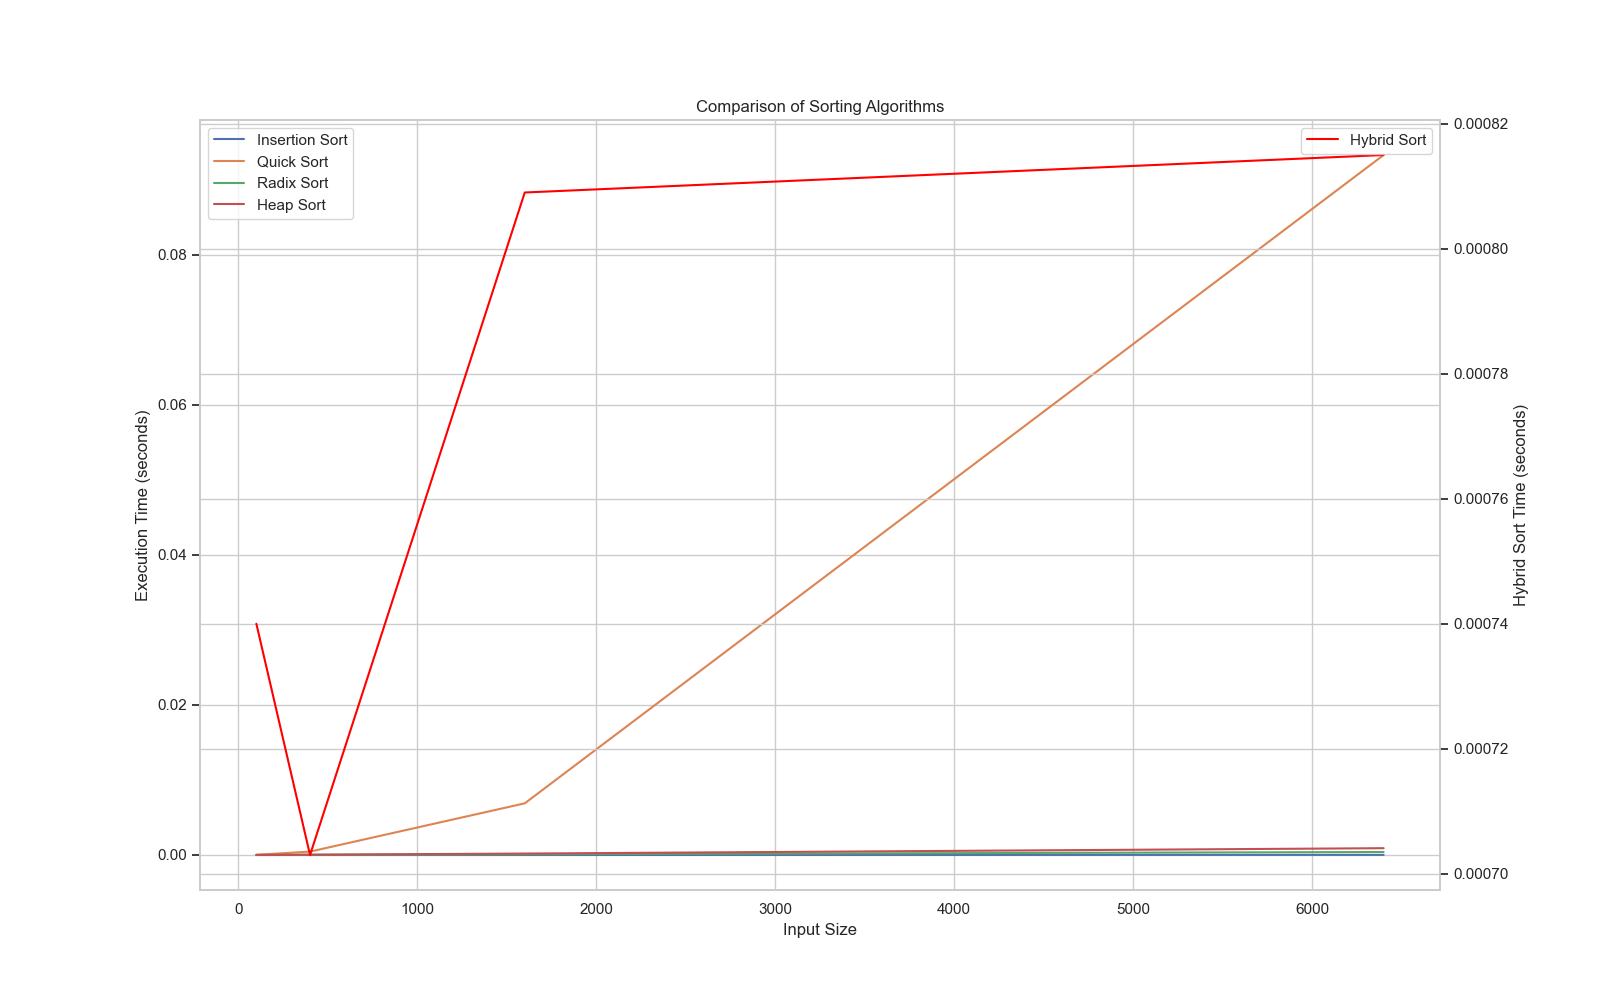
\includegraphics[width=0.8\textwidth]{../graph/all_algorithms.png}
\caption{Average time each algorithm took to sort an array of sorted values.}
\label{avg:best}
\end{figure}

\begin{figure}[h]
\centering
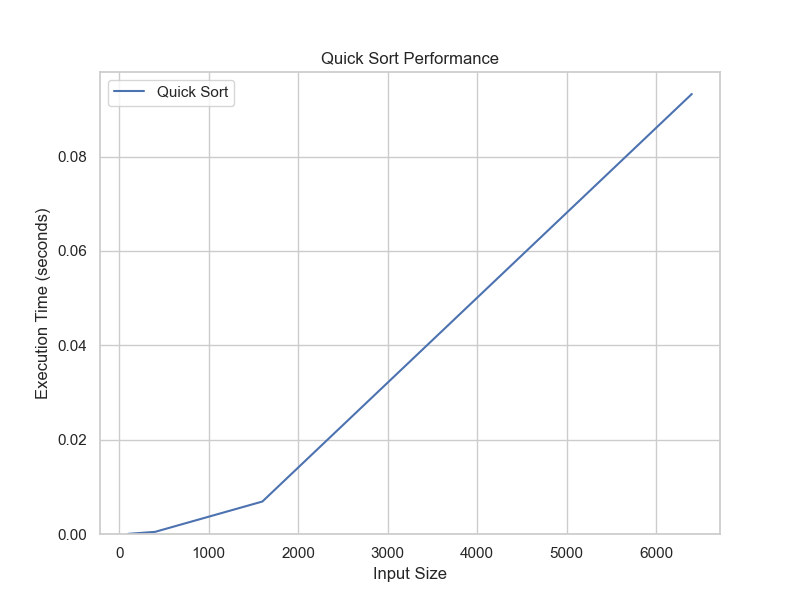
\includegraphics[width=0.8\textwidth]{../graph/quick_sort.png}
\caption{Time complexty of quicksort.}
\label{avg:best}
\end{figure}


\begin{figure}[h]
\centering
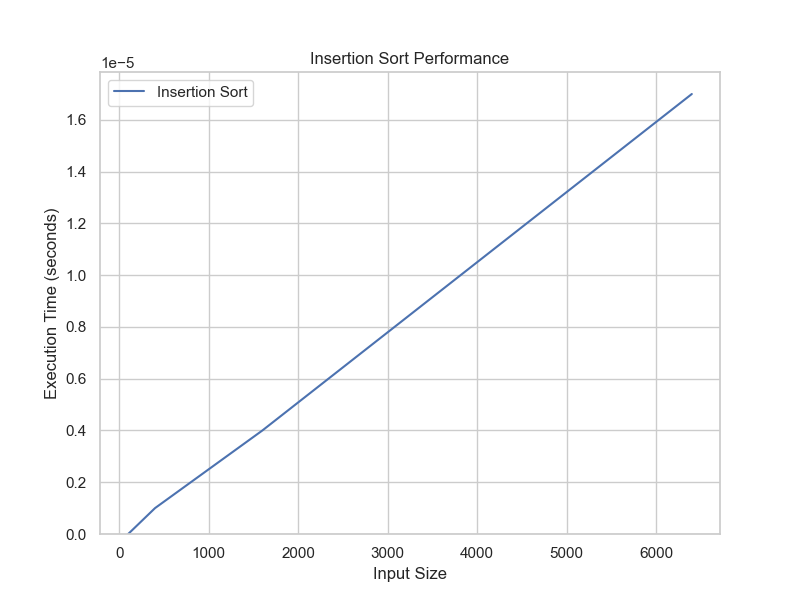
\includegraphics[width=0.8\textwidth]{../graph/insertion_sort.png}
\caption{Time complexty of insertionsort.}
\label{avg:best}
\end{figure}


\begin{figure}[h]
\centering
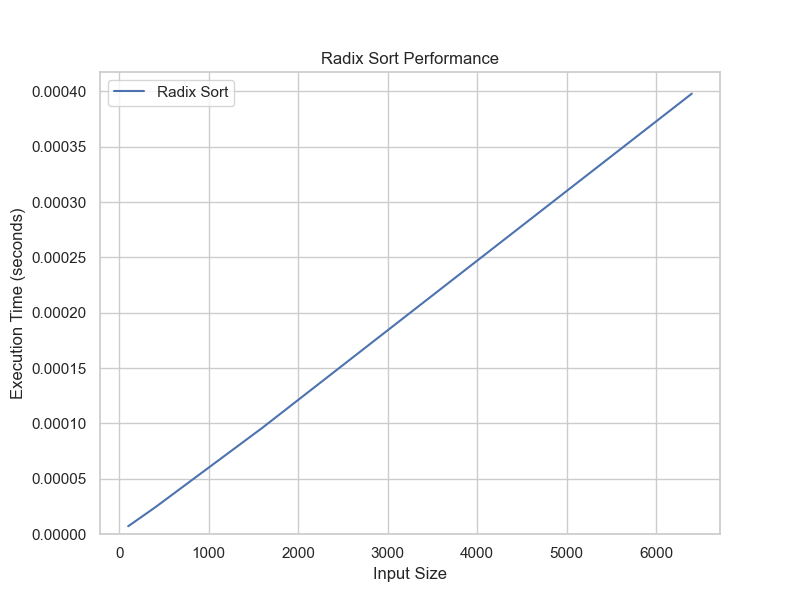
\includegraphics[width=0.8\textwidth]{../graph/radix_sort.png}
\caption{Time complexty of radixsort.}
\label{avg:best}
\end{figure}

\begin{figure}[h]
\centering
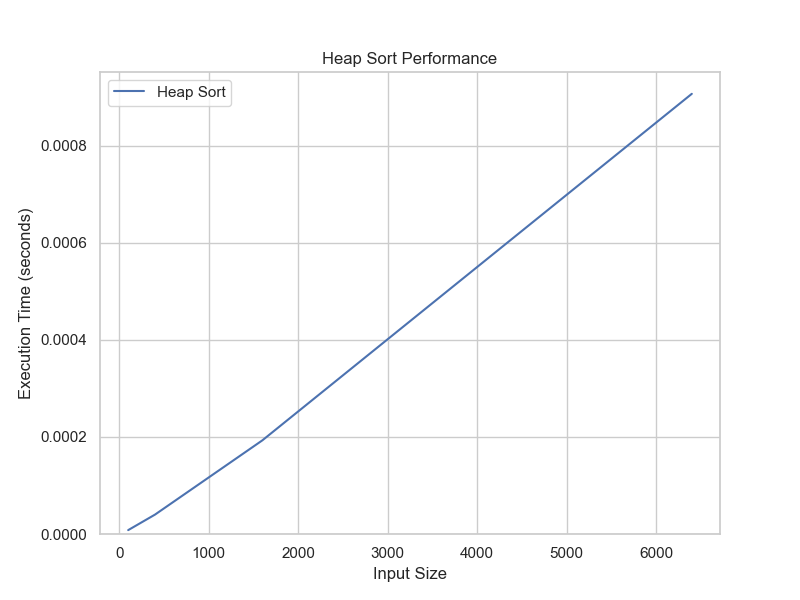
\includegraphics[width=0.8\textwidth]{../graph/heap_sort.png}
\caption{Time complexty of heapsort.}
\label{avg:best}
\end{figure}






\end{document}